\documentclass[aspectratio=169]{beamer}%页面比例16:9
\setbeamercovered{dynamic}%半透明显示
\setbeamertemplate{navigation symbols}{}
\usepackage[backend=bibtex,sorting=none,style=numeric]{biblatex}%设置引用
\addbibresource{ref.bib} %bib数据文件位置
\usepackage{dashrule}
\definecolor{NJUPurple}{rgb}{0.28235, 0.28235, 0.62745}%设置主题颜色
\colorlet{LightNJUPurple}{white!60!NJUPurple}
\colorlet{SuperLightNJUPurple}{white!90!NJUPurple}
\usecolortheme[named=NJUPurple]{structure}
\usepackage[utf8]{inputenc}
\usepackage{graphicx} % Allows including images
\usepackage{booktabs} % Allows the use of \toprule, \midrule and \bottomrule in tables
\usepackage{subfigure}
\usepackage{subfiles}
\usepackage{url}
\usepackage{amssymb}
\usepackage{amsmath}
\usepackage{xcolor,colortbl}
\usepackage[AutoFakeBold, AutoFakeSlant]{xeCJK}
\usefonttheme[onlymath]{serif}
\renewcommand{\today}{\number\year .\number\month .\number\day }

\setbeamertemplate{blocks}[rounded][shadow=true]
\setbeamercolor{block title}{fg=white,bg=NJUPurple}
\setbeamercolor{block body}{fg=black,bg=white}
\setbeamerfont{title}{shape=\bfseries,size=\Large}
\setbeamerfont{author}{shape=\bfseries}

\setbeamercolor{bibliography item}{fg = NJUPurple}
\setbeamercolor{bibliography entry title}{fg = black}
\setbeamercolor{bibliography entry author}{fg = black}
\setbeamercolor{bibliography entry location}{fg = black}
\setbeamercolor{bibliography entry note}{fg = black}

\makeatletter
    \def\@makefnmark{\hbox{{{\usebeamercolor[fg]{footnote mark}\usebeamerfont*{footnote mark} [\@thefnmark]}}}}
    \def\@makefntext#1{%
        \def\insertfootnotetext{ #1}%
        \def\insertfootnotemark{{\hbox{{{\usebeamercolor[NJUPurple]{footnote mark}\usebeamerfont*{footnote mark} [\@thefnmark]}}}}}%
        \usebeamertemplate***{footnote}}    
\makeatother
\renewcommand\footnoterule{\color{NJUPurple}\hdashrule{14cm}{1pt}{1.5mm 2pt} }
\setbeamertemplate{footnote}{
    \vspace{0.05cm}
    \scriptsize\insertfootnotemark\vspace{-0.38cm}\quad\ \insertfootnotetext\vspace{0.008cm}
}

\setbeamertemplate{title page}{%
	\vbox{}
	\vfill
	\begingroup
	\centering
	\begin{beamercolorbox}[sep=8pt,center]{title}
		\usebeamerfont{title}\inserttitle\par%
		\ifx\insertsubtitle\@empty%
		\else%
		\vskip0.25em%
		{\usebeamerfont{subtitle}\usebeamercolor[fg]{subtitle}\insertsubtitle\par}%
		\fi%     
	\end{beamercolorbox}%

	\vskip-0.2cm%<- changed
	\begin{beamercolorbox}[sep=8pt,center]{institute}
		\usebeamerfont{institute}\insertinstitute
	\end{beamercolorbox}

	\vskip-0.2cm%<- changed
	\begin{beamercolorbox}[sep=8pt,center]{author}
		\usebeamerfont{author}\insertauthor
	\end{beamercolorbox}

	\vskip-0.2cm%<- changed
	\begin{beamercolorbox}[sep=8pt,center]{date}
		\usebeamerfont{date}\insertdate
	\end{beamercolorbox}%
	\vskip0.5cm%<- changed
	
	\endgroup
	%  \vfill%<- removed
}
\makeatother

% shape, colour of item, nested item bullets in itemize only
\setbeamertemplate{itemize item}[circle] \setbeamercolor{itemize item}{fg=NJUPurple}
\setbeamertemplate{itemize subitem}[circle] \setbeamercolor{itemize subitem}{fg=NJUPurple}
\setbeamertemplate{itemize subsubitem}[circle] \setbeamercolor{itemize subsubitem}{fg=NJUPurple}

\setbeamertemplate{itemize/enumerate body begin}{\normalsize}
\setbeamertemplate{itemize/enumerate subbody begin}{\normalsize}
\setbeamertemplate{itemize/enumerate subsubbody begin}{\normalsize}

\setbeamertemplate{frametitle}
{\leavevmode%
	\begin{beamercolorbox}[wd=\paperwidth, ht=3.8ex, dp=0ex, leftskip = 1.9ex]{titlelike}%
		\usebeamerfont{frametitle}\insertframetitle\hspace{0.2cm}\usebeamerfont{framesubtitle}\insertframesubtitle%
	\end{beamercolorbox}%
}
\setbeamertemplate{section in toc}[circle] % 目录前设置序号 
\setbeamerfont{frametitle}{series=\bfseries}% 标题加粗
\setbeamerfont{framesubtitle}{size=\fontsize{11}{11},series=\bfseries}
\usepackage{latexsym,amsmath,xcolor,multicol,booktabs,calligra}
\usepackage{graphicx,pstricks,listings,stackengine}
\usepackage{wasysym}

%Contents before every section's starting slide
\AtBeginSection[]
{
	\begin{frame}
		\frametitle{Outline}
		\tableofcontents[
		currentsection,
		currentsubsection,
		subsectionstyle=show/show/hide,
		sectionstyle=show/shaded
		]
	\end{frame}
}

% 首页修改
\title{Your Title Your Title Your Title Your Title Your Title Your Title Your Title }
\subtitle{Conference 2024}
\institute{Your Institution}
\author{汇报人:君の名は}
\date{\today}

% 脚注修改
\defbeamertemplate{footline}{NGEGFootlineTemplate}{%
	\leavevmode% 离开vmode,也就是离开竖直模式,进入水平模式
 		\begin{beamercolorbox}[wd=0.975\paperwidth,ht=2.25ex,dp=3ex,right]{title in head/foot}%
			\ifnum \the\value{page}>1 \text{\href{http://www.lamda.nju.edu.cn}{http://www.lamda.nju.edu.cn}}\fi
		\end{beamercolorbox}%
%	\vskip0pt%
}
\setbeamertemplate{footline}[NGEGFootlineTemplate]
%+++++++++++++++++++++++++++++++++++正文开始+++++++++++++++++++++++++++++++++++%
\begin{document}
{
	\usebackgroundtemplate{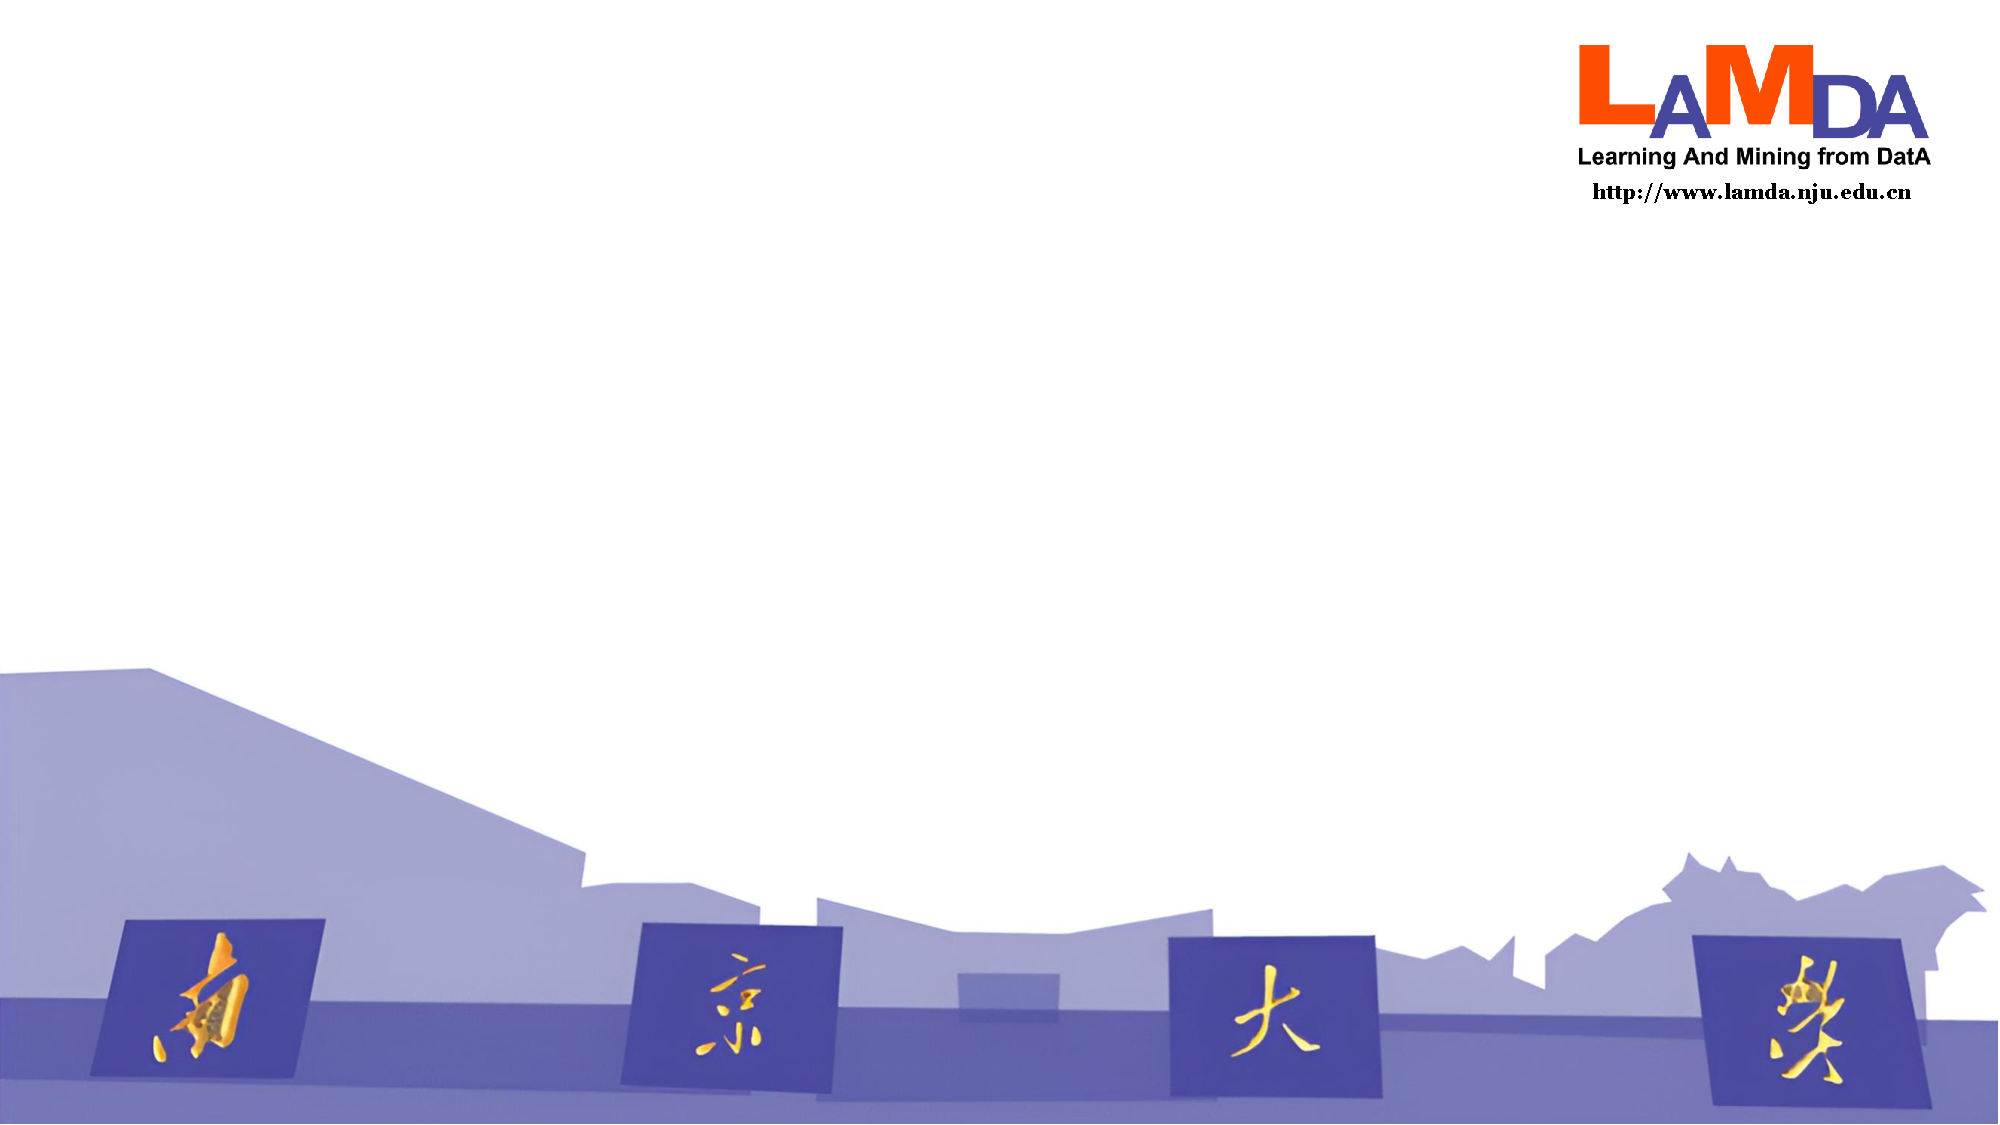
\includegraphics[width=\paperwidth,height=\paperheight]{figs/cover.pdf}}
	\frame{\titlepage}
}
{
	\usebackgroundtemplate{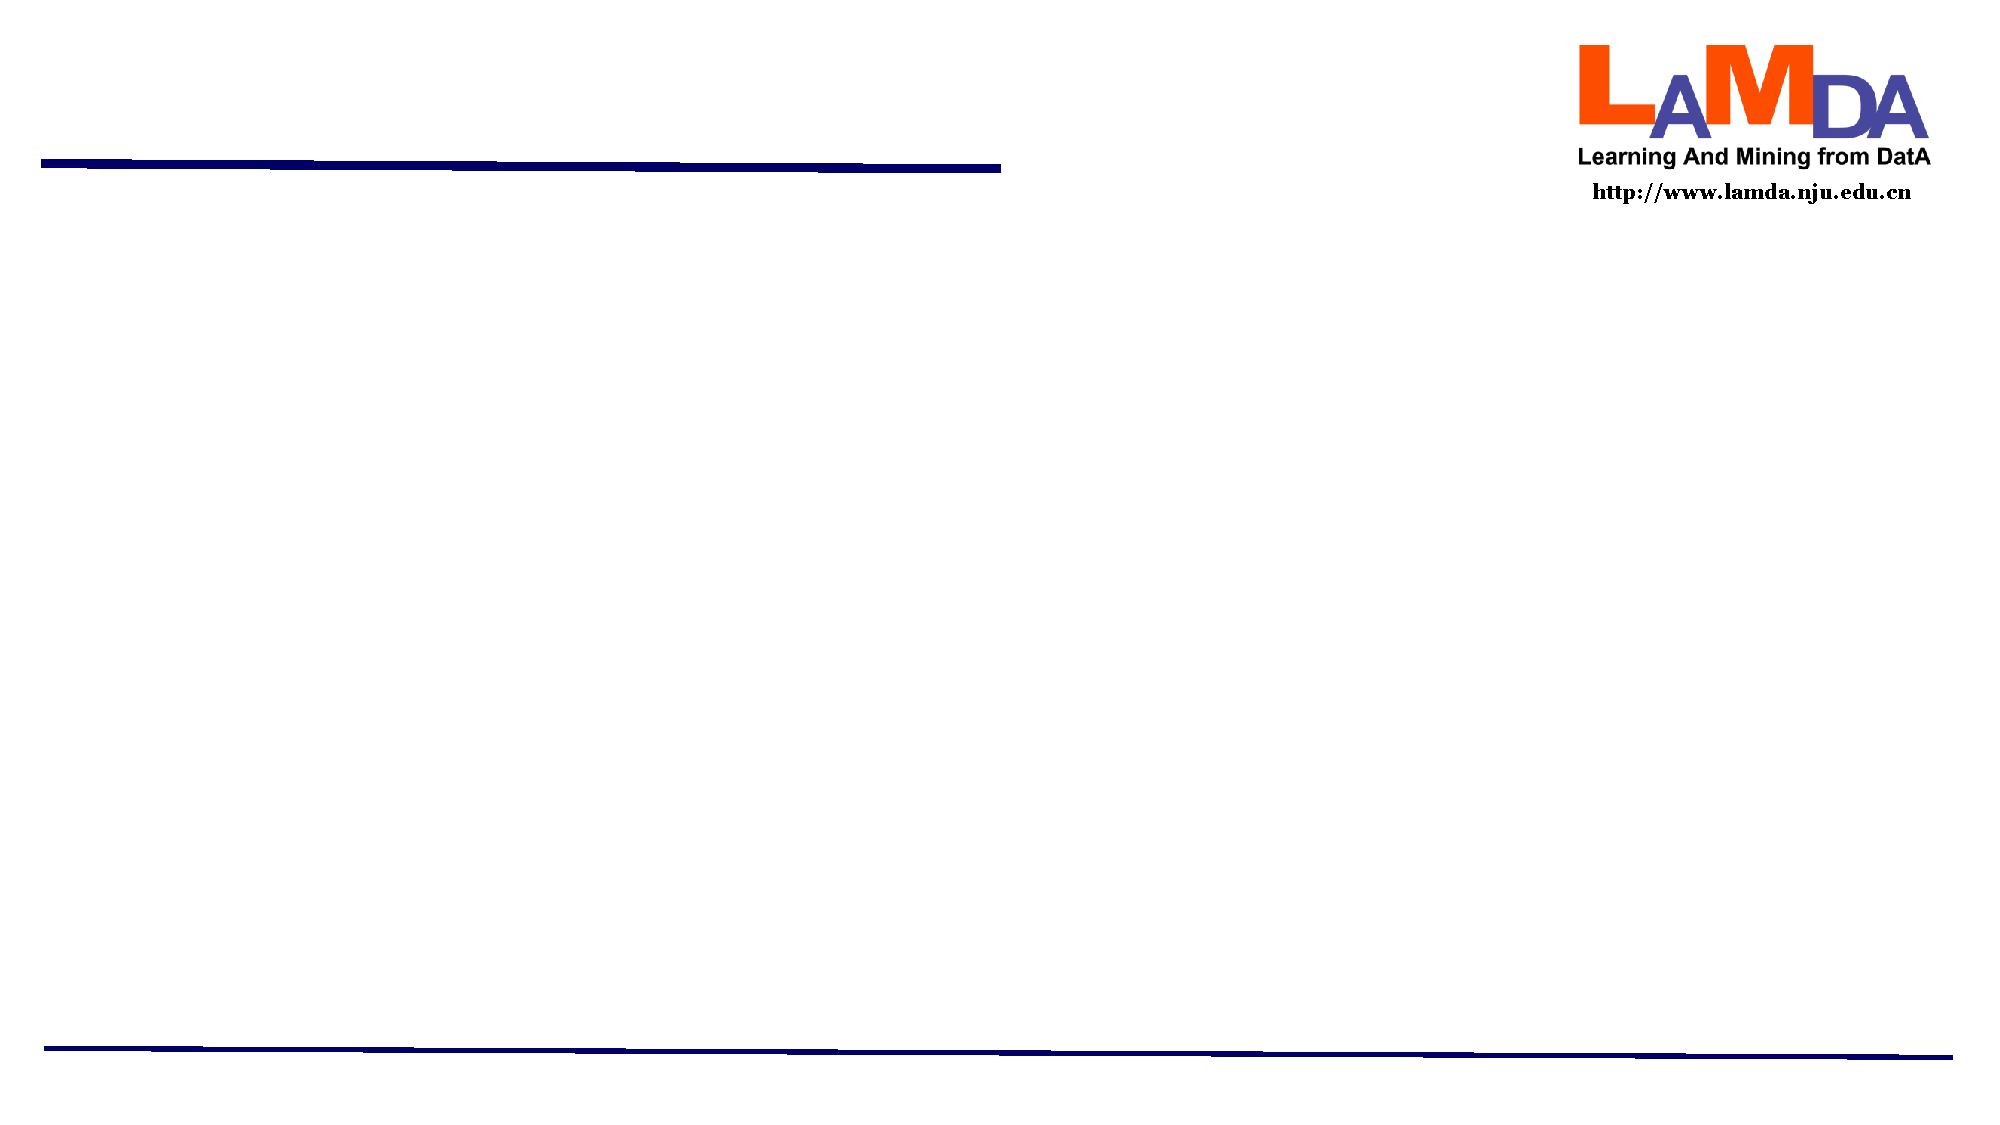
\includegraphics[width=\paperwidth,height=\paperheight]{figs/content.pdf}}

\begin{frame}
	\frametitle{About the Author(分栏显示)}
    \begin{columns}
        \begin{column}{0.37\linewidth}
            \begin{figure}
                {
\includegraphics[scale=0.16]{figs/profile.jpg}}
            \end{figure}
            {\scriptsize
             {\textbf{LinaBell}}\\Research Fellow in Nanjing University, a member of LAMDA. 
             }
        \end{column}
        \begin{column}{0.65\linewidth}
        \textbf{Latest works}
        \begin{itemize}
            \item NeurPIS
            \item ICML
            \item ICLR
            \item TPAMI
            \item PRML
        \end{itemize}
      \end{column}
  \end{columns}
\end{frame}

% 储备知识部分
\section{Preliminary}  
\begin{frame}
    \frametitle{Preliminary(公式展示)}
    \begin{itemize}
        \item{\textbf{Learning Strategy}}
        \\ \hspace*{\fill} \\
        Optimization methods:
        Pointwise loss (binary cross-entropy, mean square error), pairwise loss (BPR, WARP), and {\color{red}softmax loss}
        \begin{gather}
            \mathcal{L}_0 = -\sum_{(u,i)\in{O}^{+}}\log\frac{\exp{(\cos(\hat{\theta}_{ui})/\tau)}}{\exp{(\cos(\hat{\theta}_{ui})/\tau)}+\sum_{j\in{N}_{u}}\exp{(\cos(\hat{\theta}_{uj})/\tau)}},
            \nonumber
        \end{gather}
    \end{itemize}
\end{frame}

% 相关工作
\section{Related Work}  
    \begin{frame}
        \frametitle{Related Work(多级列表)}
        \textbf{SOTA debiasing strategies}
        \begin{itemize}
        \item
        \textbf{Sample re-weighting methods} (e.g. IPS-CN)\\
        exploit the item popularity's inverse to re-weight loss of each instance.
        \item
        \textbf{Causal inference methods} (e.g. MACR, CausE)\\
        \begin{itemize}
        \item
        specify the role of popularity bias in assumed causal
        graphs 
        \item
        mitigate the bias effect on the prediction.
        \end{itemize}
        \item
        {
        \textbf{Regularization-based frameworks} (e.g. Sam-reg) \\
        \begin{itemize}
            \item Provides a tunable mechanism for controlling the trade-off between recommendation accuracy and coverage.\\
            \item
                 \textbf{Sam-reg} regularizes the biased correlation between user-item relevance and item popularity
        \end{itemize}}
        \end{itemize}
    \end{frame}

% 方法部分
\section{Methodology}  
\subsection{BC Loss}
\begin{frame}
    \frametitle{Methodology of BC Loss}
    \framesubtitle{BC Loss(二级标题)}
    \begin{itemize}
        \item
            \textbf{BC Loss}
            \begin{align}\label{equ:bc_loss}
                \mathcal{L}_{\text{BC}} =
                -\sum_{(u,i)\in{O}^{+}}\log\frac{\exp{(\cos(\hat{\theta}_{ui}{\color{red}+M_{ui}})/\tau)}}{\exp{(\cos(\hat{\theta}_{ui}{\color{red}+M_{ui}})/\tau)}+\sum_{j\in{N}_{u}}\exp{(\cos(\hat{\theta}_{uj})/\tau)}},
                \nonumber
            \end{align}
            $M_{ui}$: the bias-aware angular margin for the interaction $(u,i)$ 
            $$M_{ui} = \min \{\hat{\xi}_{ui}, \pi - \hat{\theta}_{ui}\}$$
        \item\textbf{Intuition}\\
                If a user-item pair is the hard interaction that can hardly be reconstructed by its popularity statistics, it holds a
        high value of $\xi_{ui}$ and leads to a high value of $M_{ui}$. Henceforward, BC loss imposes the large angular
        margin $M_{ui}$ between the negative item $j$ and positive item $i$.
    \end{itemize}
\end{frame}

% 分析部分
\section{Analyses}  
    \subsection{Geometric Interpretation}
        \begin{frame}
            \frametitle{Analyses(图像展示)}
            \framesubtitle{Geometric Interpretation}
            \begin{itemize}
            \item
                \textbf{Geometric Interpretation}\\
                    User $u$ with one observed item $i$ and two unobserved items $j$ and $k$.\\
                    \begin{figure}
                        {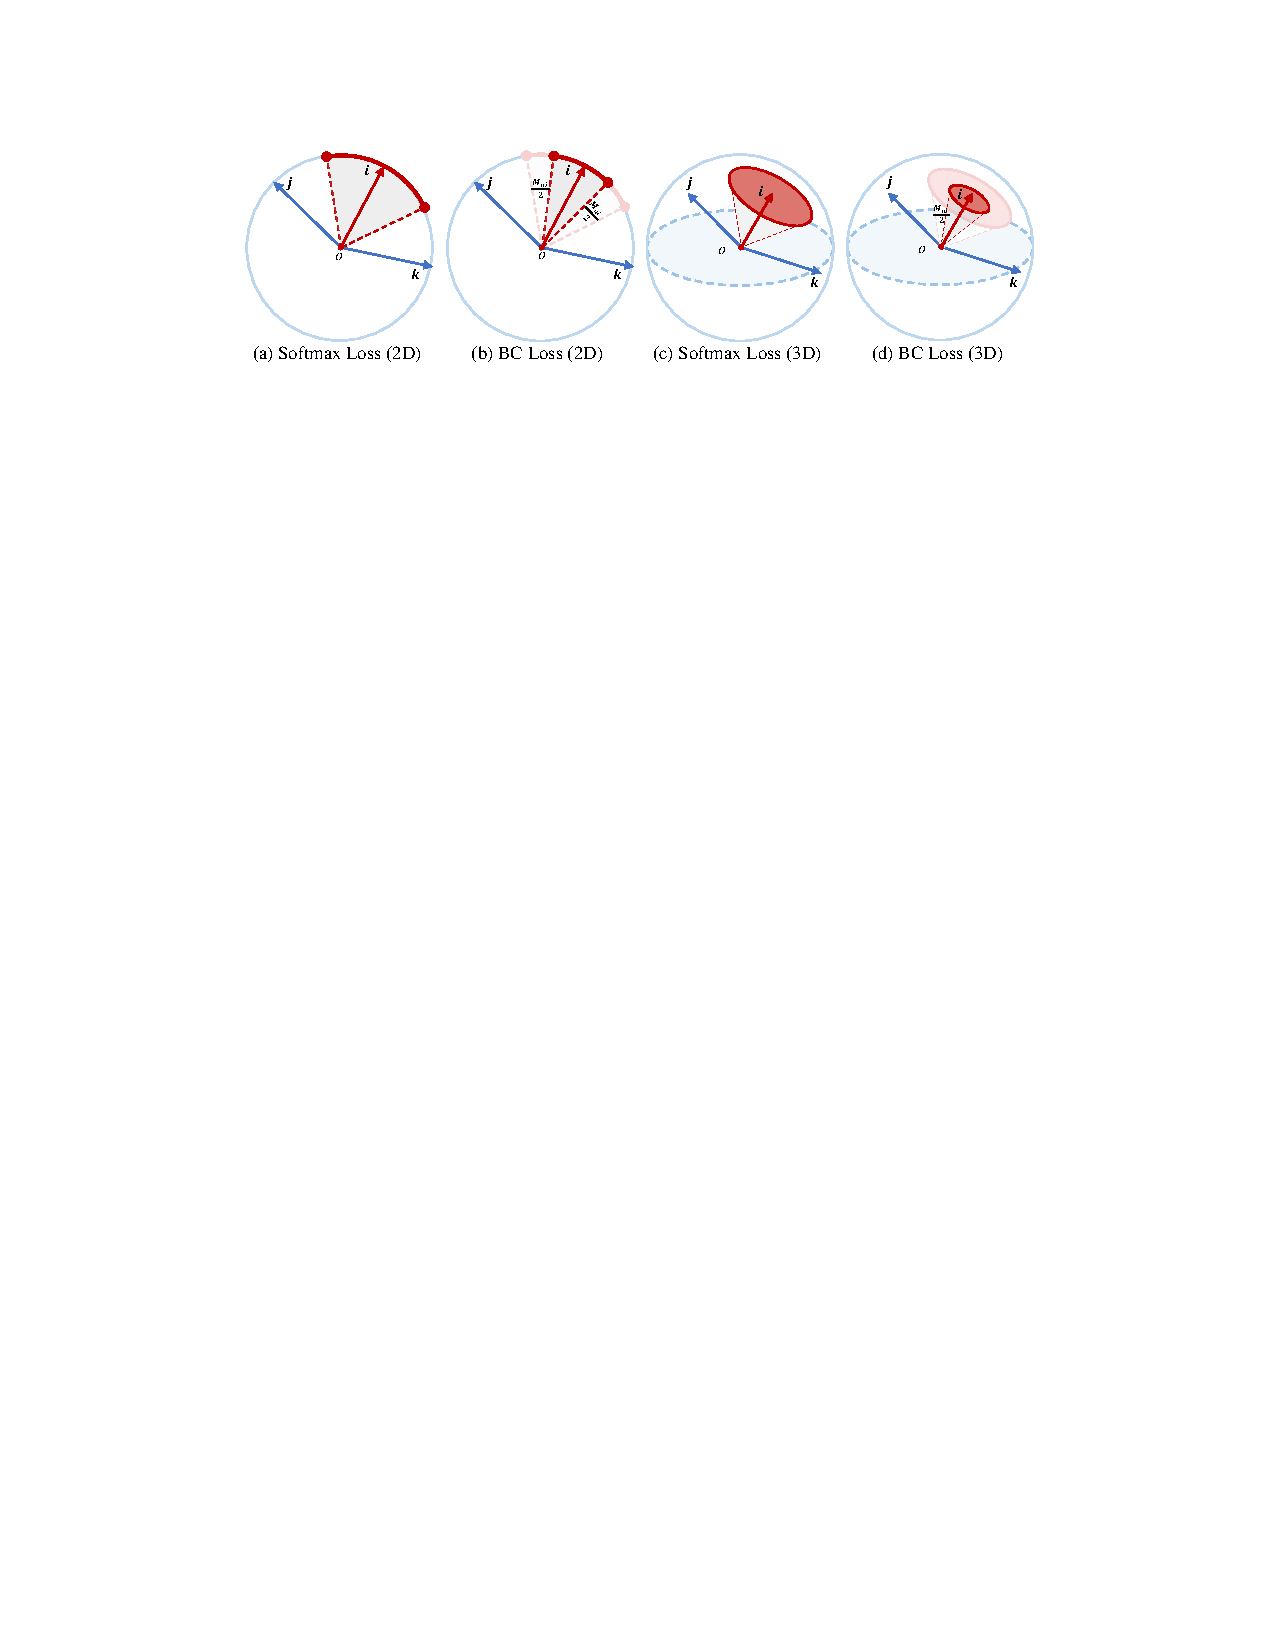
\includegraphics[scale=0.92]{figs/fig.pdf}}
                    \end{figure}
            \end{itemize}
        \end{frame}

    \subsection{Theoretical Properties}
         \begin{frame}
            \frametitle{Analyses(数学环境)}
            \framesubtitle{Theoretical Properties}
            \begin{itemize}
            \item
            \textbf{Theoretical Properties}
            \begin{proof}
            1. There exists an upper bound $m$, s.t. $-1 < \cos(\hat{\theta}_{ui}+M_{ui}) \leq {v}_u^T{v}_i - m <  1 $\\
            2. \\
            3. \\
            4. \\
            5. \\
            6. \\

            \end{proof}
            \end{itemize}
        \end{frame}

% 实验部分
\section{Experiments}  
\begin{frame}
    	\frametitle{Experiments(表格展示)}
         \framesubtitle{Baselines \& Datasets}
         \textbf{Baselines}
         \begin{itemize}
         \item
            Backbone: only use softmax loss
            \item
            IPS-CN: sample re-weighting methods
            \item
            CausE: bias removal by causal inference
            \item
            sam + reg: regularization-based framework
            \item
            MACR: bias removal by causal inference
        \end{itemize}
        \textbf{Datasets}
            \resizebox{\columnwidth}{!}{
            \begin{tabular}{lrrrrrrr}
            \toprule
             & KuaiRec & Douban Movie & Tencent & Amazon-Book & Alibaba-iFashion & Yahoo!R3 & Coat\\ \midrule
            \#Users & 7175 & 36,644 & 95,709 & 52,643 & 300,000 & 14382 & 290 \\
            \#Items & 10611 & 22,226 & 41,602 & 91,599 & 81,614 & 1000 & 295 \\
            \#Interactions & 1062969 & 5,397,926 & 2,937,228 & 2,984,108 & 1,607,813 & 129,748 & 2,776 \\
            Sparsity & 0.01396 & 0.00663 & 0.00074 & 0.00062 & 0.00007 
            & 0.00902 &  0.03245\\  \bottomrule
            \end{tabular}}
    \end{frame}

% 结论部分
 \section{Conclusion}  
    \begin{frame}
        \frametitle{Conclusion(脚注使用)}
        \begin{itemize}
            \item
            \textbf{Contribution}\\
            \begin{itemize}
                \item
                (Originality) Popular bias extractor has an intuitive geometric interpretation.
                \item
                (Quality) Outperforms existing methods in various evaluation protocols.
                \item
                (Clarity) Well-written and easy to understand. Theoretical proof is quite solid.
            \end{itemize}
            \item
            \textbf{Limitation}\\
            \begin{itemize}
                \item
                The technical contribution of this paper is limited.It only proposes to employ an extra popularity-based predictor and combine the results with an existing CF model\footfullcite{he2020momentum}.
                \item
                Overclaims the strength of the proposed BC loss in theoretical analysis. The geometric interpretability and the hard-negative mining ability are actually the same thing\parencite{ pmlr-v119-wang20k, yuan2021one}
            \end{itemize}
        \end{itemize}
    \end{frame}

% 引用部分
\section*{References}
	\begin{frame}[allowframebreaks]
	\frametitle{References}\color{NJUPurple}{
        \printbibliography[heading=none]}
	\end{frame}

% 谢辞部分
\section*{Acknowledgement}  
    \begin{frame}
        \frametitle{Acknowledgement}
        \textcolor{NJUPurple}{\Huge{\centerline{Thank you!}}}
    \end{frame}
}

\end{document}